% defer/hazptr.tex
% Can I hazptr cheezeberger?

\section{Hazard Pointers}
\label{sec:defer:Hazard Pointers}

One way of avoiding problems with concurrent reference counting
is to implement the reference counters
inside out, that is, rather than incrementing an integer stored in the
data element, instead store a pointer to that data element in
per-CPU (or per-thread) lists.
Each element of these lists is called a
\emph{hazard pointer}~\cite{MagedMichael04a}.\footnote{
	Also independently invented by others~\cite{HerlihyLM02}.}
The value of a given data element's ``virtual reference counter'' can
then be obtained by counting the number of hazard pointers referencing
that element.
Therefore, if that element has been rendered inaccessible to readers,
and there are no longer any hazard pointers referencing it, that element
may safely be freed.

{ \scriptsize
\begin{verbbox}
 1 int hp_store(void **p, void **hp)
 2 {
 3   void *tmp;
 4 
 5   tmp = ACCESS_ONCE(*p);
 6   ACCESS_ONCE(*hp) = tmp;
 7   smp_mb();
 8   if (tmp != ACCESS_ONCE(*p) ||
 9       tmp == HAZPTR_POISON) {
10     ACCESS_ONCE(*hp) = NULL;
11     return 0;
12   }
13   return 1;
14 }
15 
16 void hp_erase(void **hp)
17 {
18   smp_mb();
19   ACCESS_ONCE(*hp) = NULL;
20   hp_free(hp);
21 }
\end{verbbox}
}
\begin{figure}[btp]
\centering
\theverbbox
\caption{Hazard-Pointer Storage and Erasure}
\label{fig:defer:Hazard-Pointer Storage and Erasure}
\end{figure}

Of course, this means that hazard-pointer acquisition must be carried
out quite carefully in order to avoid destructive races with concurrent
deletion.
One implementation is shown in
Figure~\ref{fig:defer:Hazard-Pointer Storage and Erasure},
which shows \co{hp_store()} on lines~1-13 and \co{hp_erase()} on
lines~15-20.
The \co{smp_mb()} primitive will be described in detail in
Section~\ref{sec:advsync:Memory Barriers}, but may be ignored for
the purposes of this brief overview.

The \co{hp_store()} function records a hazard pointer at \co{hp} for the data
element whose pointer is referenced by \co{p}, while checking for
concurrent modifications.
If a concurrent modification occurred, \co{hp_store()} refuses to record
a hazard pointer, and returns zero to indicate that the caller must
restart its traversal from the beginning.
Otherwise, \co{hp_store()} returns one to indicate that it successfully
recorded a hazard pointer for the data element.

\QuickQuiz{}
	Why does \co{hp_store()} in
	Figure~\ref{fig:defer:Hazard-Pointer Storage and Erasure}
	take a double indirection to the data element?
	Why not \co{void *} instead of \co{void **}?
\QuickQuizAnswer{
	Because \co{hp_record()} must check for concurrent modifications.
	To do that job, it needs a pointer to a pointer to the element,
	so that it can check for a modification to the pointer to the
	element.
} \QuickQuizEnd

\QuickQuiz{}
	Why does \co{hp_store()}'s caller need to restart its
	traversal from the beginning in case of failure?
	Isn't that inefficient for large data structures?
\QuickQuizAnswer{
	It might be inefficient in some sense, but the fact is that
	such restarting is absolutely required for correctness.
	To see this, consider a hazard-pointer-protected linked list
	containing elements~A, B, and~C that is subjecte to the
	following sequence of events:

	\begin{enumerate}
	\item	Thread~0 stores a hazard pointer to element~B
		(having presumably traversed to element~B from element~A).
	\item	Thread~1 removes element~B from the list, which sets
		the pointer from element~B to element~C to a special
		\co{HAZPTR_POISON} value in order to mark the deletion.
		Because Thread~0 has a hazard pointer to element~B,
		it cannot yet be freed.
	\item	Thread~1 removes element~C from the list.
		Because there are no hazard pointers referencing element~C,
		it is immediately freed.
	\item	Thread~0 attempts to acquire a hazard pointer to
		now-removed element~B's successor, but sees the
		\co{HAZPTR_POISON} value, and thus returns zero,
		forcing the caller to restart its traversal from the
		beginning of the list.
	\end{enumerate}

	Which is a very good thing, because otherwise Thread~0 would
	have attempted to access the now-freed element~C,
	which might have resulted in arbitrarily horrible
	memory corruption, especially if the memory for
	element~C had since been re-allocated for some other
	purpose.

	All that aside, please understand that hazard pointers's
	restarting allows it to maintain a minimal memory footprint.
	Any object not currently referenced by some hazard pointer
	may be immediately freed.
	In contrast,
	Section~\ref{sec:defer:Read-Copy Update (RCU)}
	will discuss a mechanism that avoids read-side retries
	(and minimizes read-side overhead), but has a much larger
	memory footprint.
} \QuickQuizEnd

\QuickQuiz{}
	Given that papers on hazard pointers use the bottom bits
	of each pointer to mark deleted elements, what is up with
	\co{HAZPTR_POISON}?
\QuickQuizAnswer{
	The published implementations of hazard pointers used
	non-blocking synchornization techniques for insertion
	and deletion.
	These techniques require that readers traversing the
	data structure ``help'' updaters complete their updates,
	which in turn means that readers need to look at the successor
	of a deleted element.

	In contrast, we will be using locking to synchronize updates,
	which does away with the need for readers to help updaters
	complete their updates, which in turn allows us to leave
	pointers' bottom bits alone.
	This approach allows read-side code to be simpler and faster.
} \QuickQuizEnd

Because algorithms using hazard pointers might be restarted at any
step of their traversal through the data structure, such algorithms
must typically take care to avoid making any changes to the data
structure until after they have acquired all relevant hazard pointers.

\QuickQuiz{}
	But don't these restrictions on hazard pointers also apply
	to other forms of reference counting?
\QuickQuizAnswer{
	These restrictions apply only to reference-counting mechanisms whose
	reference acquisition can fail.
} \QuickQuizEnd

These restrictions result in great benefits to readers, courtesy of the
fact that the hazard pointers are stored local to each CPU/thread,
which in turn allows traversals of the data structures themselves to
be carried out in a completely read-only fashion.
Referring back to
Figure~\ref{fig:count:Optimization and the Four Parallel-Programming Tasks}
on
page~\pageref{fig:count:Optimization and the Four Parallel-Programming Tasks},
hazard pointers enable the CPU caches to do resource replication, which
in turn allows weakening of the parallel-access-control mechanism,
thus boosting performance and scalability.
Performance comparisons with other mechanisms may be found in
Chapter~\ref{chp:Data Structures}
and in other publications~\cite{ThomasEHart2007a,McKenney:2013:SDS:2483852.2483867,MagedMichael04a}.

{ \scriptsize
\begin{verbbox}
 1 struct route_entry {
 2   struct hazptr_head hh;
 3   struct route_entry *re_next;
 4   unsigned long addr;
 5   unsigned long iface;
 6   int re_freed;
 7 };
 8 struct route_entry route_list;
 9 DEFINE_SPINLOCK(routelock);
10 hazard_pointer __thread *my_hazptr;
11
12 unsigned long route_lookup(unsigned long addr)
13 {
14   int offset = 0;
15   struct route_entry *rep;
16   struct route_entry **repp;
17
18 retry:
19   repp = &route_list.re_next;
20   do {
21     rep = ACCESS_ONCE(*repp);
22     if (rep == NULL)
23       return ULONG_MAX;
24     if (rep == (struct route_entry *)HAZPTR_POISON)
25       goto retry;
26     my_hazptr[offset].p = &rep->hh;
27     offset = !offset;
28     smp_mb();
29     if (ACCESS_ONCE(*repp) != rep)
30       goto retry;
31     repp = &rep->re_next;
32   } while (rep->addr != addr);
33   if (ACCESS_ONCE(rep->re_freed))
34     abort();
35   return rep->iface;
36 }
\end{verbbox}
}
\begin{figure}[bp]
\centering
\theverbbox
\caption{Hazard-Pointer Pre-BSD Routing Table Lookup}
\label{fig:defer:Hazard-Pointer Pre-BSD Routing Table Lookup}
\end{figure}

{ \scriptsize
\begin{verbbox}
 1 int route_add(unsigned long addr,
 2               unsigned long interface)
 3 {
 4   struct route_entry *rep;
 5
 6   rep = malloc(sizeof(*rep));
 7   if (!rep)
 8     return -ENOMEM;
 9   rep->addr = addr;
10   rep->iface = interface;
11   rep->re_freed = 0;
12   spin_lock(&routelock);
13   rep->re_next = route_list.re_next;
14   route_list.re_next = rep;
15   spin_unlock(&routelock);
16   return 0;
17 }
18
19 int route_del(unsigned long addr)
20 {
21   struct route_entry *rep;
22   struct route_entry **repp;
23
24   spin_lock(&routelock);
25   repp = &route_list.re_next;
26   for (;;) {
27     rep = *repp;
28     if (rep == NULL)
29       break;
30     if (rep->addr == addr) {
31       *repp = rep->re_next;
32       rep->re_next =
33           (struct route_entry *)HAZPTR_POISON;
34       spin_unlock(&routelock);
35       hazptr_free_later(&rep->hh);
36       return 0;
37     }
38     repp = &rep->re_next;
39   }
40   spin_unlock(&routelock);
41   return -ENOENT;
42 }
\end{verbbox}
}
\begin{figure}[bp]
\centering
\theverbbox
\caption{Hazard-Pointer Pre-BSD Routing Table Add/Delete}
\label{fig:defer:Hazard-Pointer Pre-BSD Routing Table Add/Delete}
\end{figure}

\begin{figure}[tb]
\centering
\resizebox{2.5in}{!}{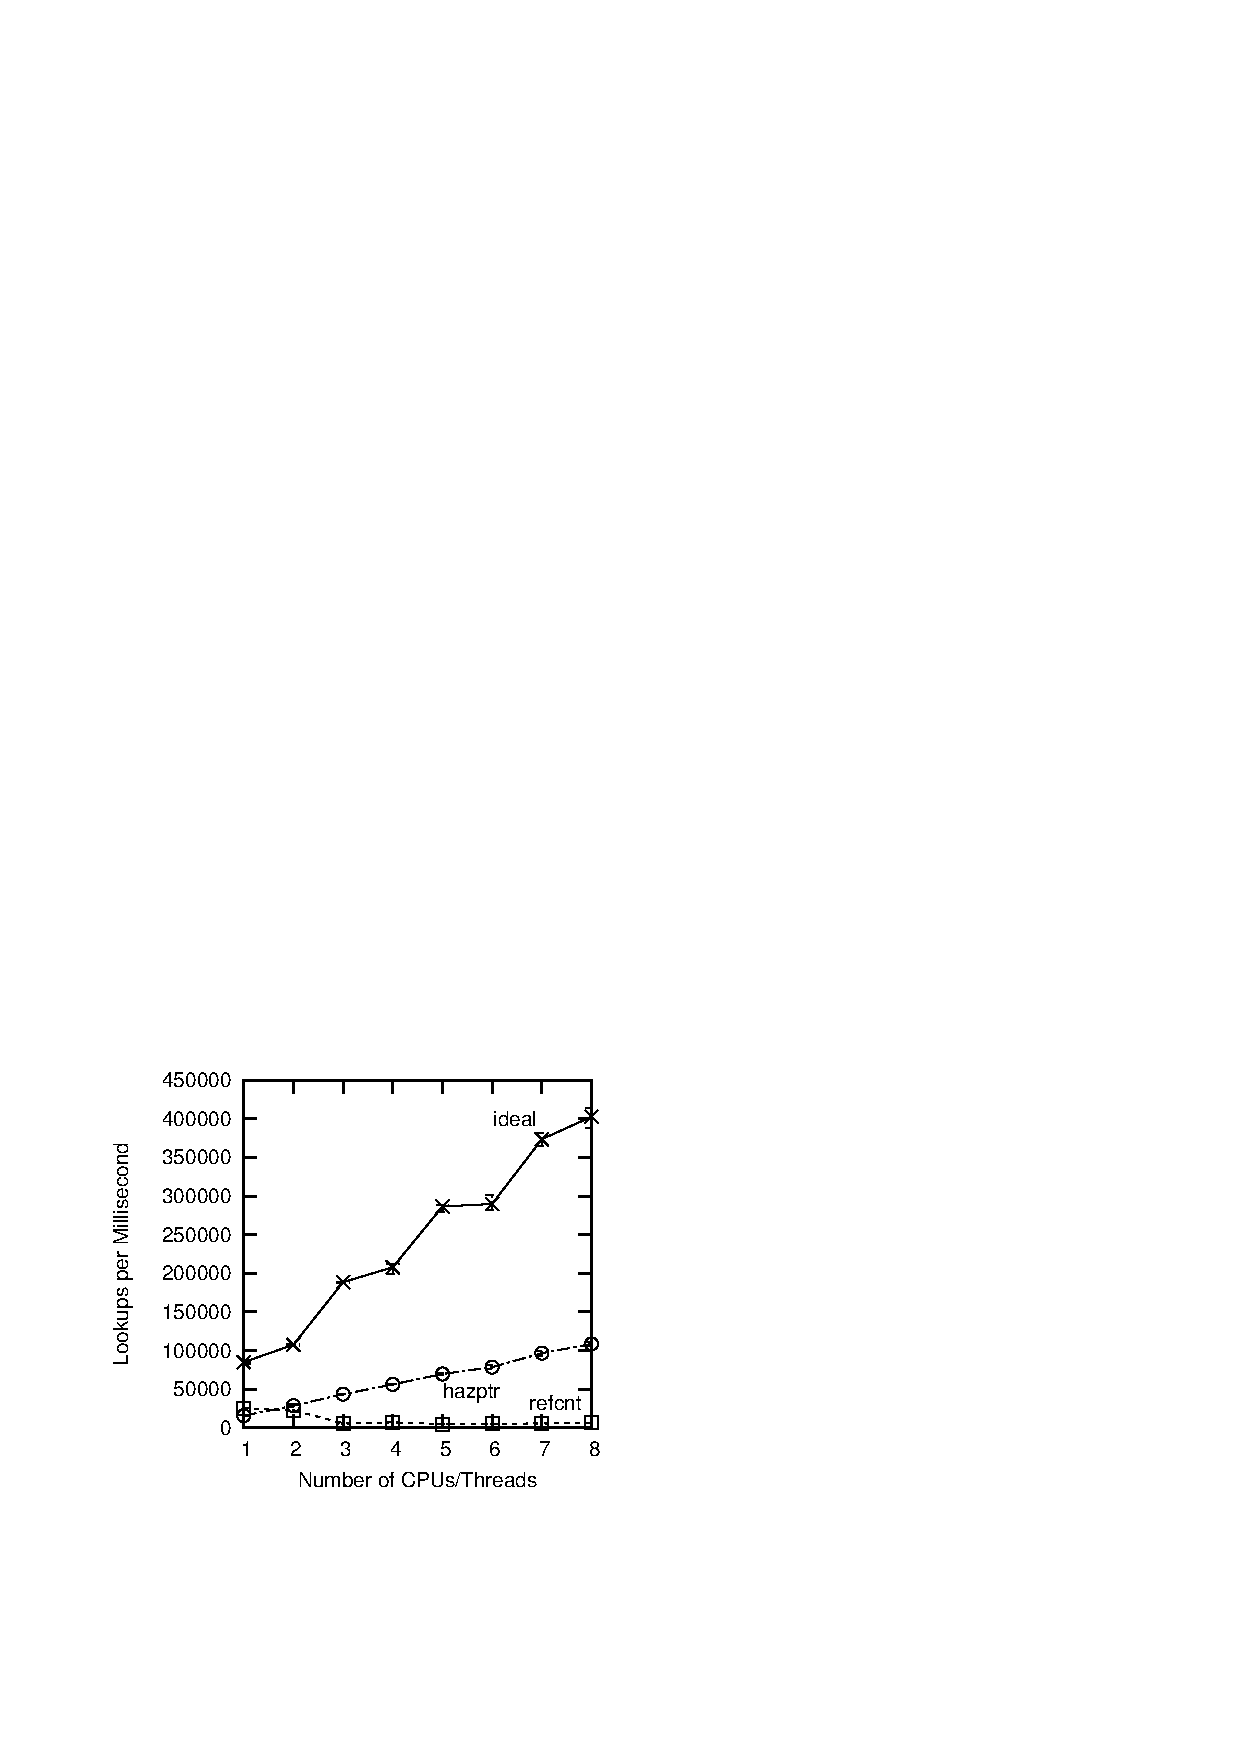
\includegraphics{CodeSamples/defer/data/paulmck.2016/perf-hazptr}}
\caption{Pre-BSD Routing Table Protected by Hazard Pointers}
\label{fig:defer:Pre-BSD Routing Table Protected by Hazard Pointers}
\end{figure}

Hazard pointers are much more scalable than reference counters,
but they still require readers to do writes to shared memory.
The topic of the next section, sequence counters, avoids read-side
writes entirely.
